\documentclass[11pt]{article}
\usepackage[usenames, dvipsnames]{color}
\usepackage[margin=1in,vmargin=1in]{geometry}
\usepackage[utf8]{inputenc}
\usepackage[english]{babel}
\usepackage{tikz}
\usepackage{pgfplots}
\usepackage{fancyhdr}
\pagestyle{fancy}
\usepackage{floatrow}
\usepackage[font=small,labelfont=bf,labelsep=period]{caption}
\usepgfplotslibrary{polar}
\usepgflibrary{shapes.geometric}
\usetikzlibrary{calc}
\pgfplotsset{compat=1.5.1}
\pgfmathdeclarefunction{gauss}{2}{%
  \pgfmathparse{1/(#2*sqrt(2*pi))*exp(-((x-#1)^2)/(2*#2^2))}%
}

\pgfmathdeclarefunction{bivar}{4}{%
  \pfgmathparse{1/(2*pi*#2*#4) * exp(-((x-#1)^2/#2^2 +
    (y-#3)^2/#4^2))/2}%
}
\usetikzlibrary{shadows}
\usepackage{graphicx}
\usepackage{graphics}
\usepackage[mode=buildnew]{standalone}
\usepackage{amsmath}
\usepackage{amsthm}
\usepackage{amssymb}
\usepackage{float}
\DeclareMathOperator*{\argmin}{arg\,min}
\newcommand*{\everymodeprime}{\ensuremath{\prime}}
\usepackage [autostyle, english = american]{csquotes}
\usepackage[backend=bibtex,sorting=none]{biblatex}
\usepackage{wrapfig}
\bibliography{Master}
\graphicspath{ {img/} {figures/} }
\definecolor{purduegold}{cmyk}{.43,.56,1,0}
\newcommand{\mcolor}[2][red]{{\color{#1}\textbf{#2}}}

\usepackage{algorithm}
\usepackage[noend]{algpseudocode}


\newcommand*\DNA{\textsc{dna}}
\newcommand*\Let[2]{\State #1 $\gets$ #2}
\title{Machine Learning Models and Algorithms Summary}
\author{Kent Gauen and Dr. Xiao Wang}
\date{}
\begin{document}
\maketitle
\tableofcontents

\section{Introduction}
\par
    Machine learning is a powerful tool used in a wide breadth of applications including quality control, image classification, and self-driving cars. We give a broad summary of many fundamental machine learning models, so that the reader may gain an intuition behind their formulation. In this paper, we use the MNIST dataset to demonstrate the mechanisms of machine learning models. There are three major teaching paradigms --  supervised, unsupervised, and semi-supervised learning. We will discuss supervied and unsupervised learning. For supervised learning, we discuss logistic regression, support vector machines, and convolutional neural networks. For unsupervised learning, we discuss the k-means cluster method, principal components analysis, and auto-encoders. Each of the methods are separated into the problem formulation, a brief overview of the algorithm. After each of the models are presented, a summary of the results is provided to compare the performance of the models. 
\par
    Note that the purpose of this paper is not to provide a comprehensive review of old methodology, introduce new methodology, or present new results. This paper's goal is to present the basics of fundamental machine learning models to a target audience of undergraduate students with a minimal statistics and mathematics background. However, we do expect the reader to be familiar with linear regression.

\section{Dataset: MNIST}
The MNIST dataset was originally black and white images from the NIST, National Institute of Standards and Technology. They are a mixture of Special Database 1 (high-school students) and Special Database 3 (Census Bureau), which are binary images of handwritten arabic integers from $0$ through $9$. The MNIST, or Mixed NIST, dataset are normalized to a $20\times20$ pixel box while preserving their aspect ration. The dataset contains $60,000$ images of digits for training, and $10,000$ images of digits for testing \cite{mnist_lecun}. 

\begin{figure}[H]
  \floatbox[{\capbeside\thisfloatsetup{capbesideposition={right},capbesidewidth=8cm}}]{figure}[\FBwidth]
  {\caption{The MNIST dataset is gray-scale images of handwritten arabic integers, $0 - 9$. This provides machine learning researchers with an easily understood dataset, demands little pre-processing, and requires a non-trivial solution.
    }\label{fig:mnist_ex}}{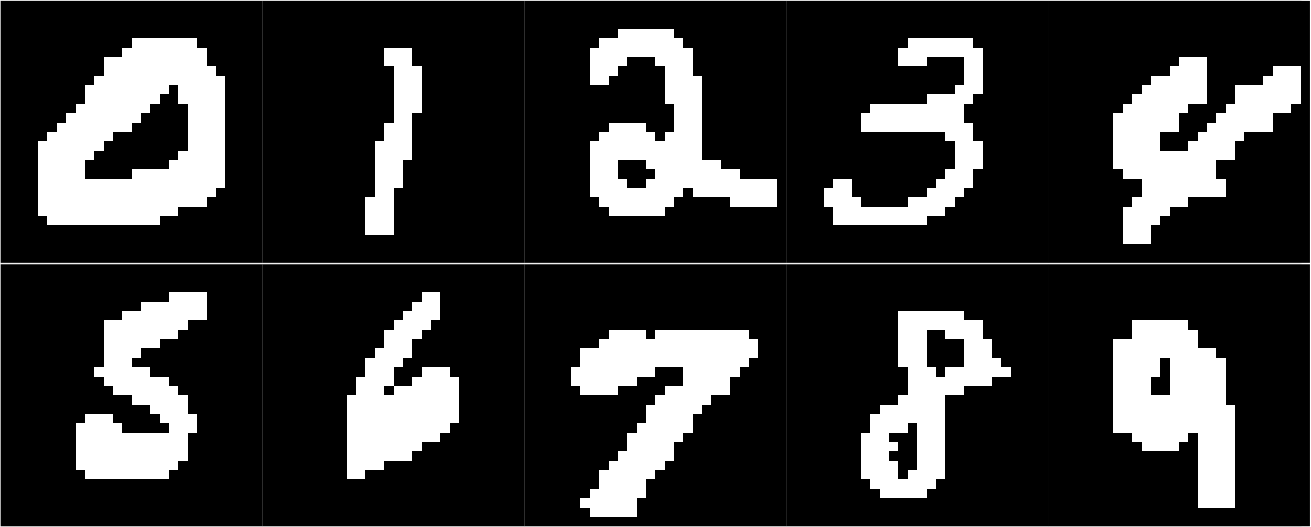
\includegraphics[width=0.3\textwidth]{img_mnist}}
\end{figure}

The MNIST dataset is widely popular for benchmarking image classification models. There is little to no pre-processing required, and the task is straight-forward: what is the digit in the image? The task is also non-trivial. For example, how do we construct a model that can recognize a $2$ shifted in an image? Linear classifiers struggle classifying shifted images. The MNIST dataset is good choice to use for this paper, given it's educational purpose.

\section{Supervised Learning}

\par
Classification is the task of determining which category, or class, an input belongs to. Classification tasks inlude any task that categorizes input features into a finite number of classes. A common classification task is image recognition; e.g. a picture's pixels are used as the input, and a model can determine if the image contains a dog, building, car, a combination of two classes, all three classes, or none of them.

In supervised classification, the data set is comprised of N samples of $\mathbf{x}$ written together as $\mathbf{X} \equiv (\mathbf{x}_{1},\ldots,\mathbf{x}_{N})$ with target values $\mathbf{t}$, written together as $\mathbf{T} \equiv (\mathbf{t}_{1},\ldots,\mathbf{t}_{N})$. The input data $\mathbf{x}$ is a column vector containing real valued features with dimensionality \textbf{D}, $\mathbf{x} = (x_{1},\ldots,x_{D})^{T}$. The data gives information to predict the target $\mathbf{t}$. While the target value can be written many ways, we will assume the target varaible will be binary column vector of \textbf{K} dimensions for a $k$ class classification problem, $\mathbf{t} = (t_{1},\ldots,t_{k})^{T}$. With the exception of support vector machines, we will pose our classification tasks such that $\sum_{i=1}^{k} t_{i} = 1$, or in words, each input only has one correct output. Relating to the image recognition task above, we will only consider cases in which an input image contains only a dog, building, car, or none of them.

We use a weight vector $\mathbf{w}$ with dimensions \textbf{D$+1$}, given our input has dimensions \textbf{D}. The extra dimension for $\mathbf{w}$ is required for a bias term $w_0$ (not to be confused with \emph{bias} the statistical term). Therefore it is assumed that our weight vectors are defined as $\mathbf{w} = (w_{0},w_{1},\ldots,w_{D})^{T}$. Our input features $\mathbf{x}$ are then re-defined as $\mathbf{x} = (1,x_{1},\ldots,x_{D})^{T}$. This format allows us to use vectorized equations instead of summations, which will clear-up our equations. 

Often we will also use $\phi(\mathbf{x})$ as a basis function for $\mathbf{x}$. Our basis functions can be written as $\phi(\mathbf{x})$ or $\phi$, but it is still a function of $\mathbf{x}$ even if the explicit dependence is omitted. It often will be omitted for less cluttered notation.

\par
In the following section we will use the neural network framework to explain (a) multilayer perceptrons, (b) logistic regression, (c) convolutional neural networks, and (d) support vector machines. 

\subsection{Multilayer Perceptrons Methodoloy \&  Analysis}

\par
Before we discuss neural networks, it is important to motivate why neural networks, and deep learning, are currently a popular topic. In image recognition, many people have studied hand-engineered features to decompose images into fundamental building blocks. These processes include SIFT, GLOH, Spin Image, HoG, Textons, and RIFT. While the results are moderately effective, the process of constructing hand-engineered features is slow. Deep learning is attractive because it allows us to construct better features \emph{automatically}. The most recent milestone is Alex Krizhevsky's 2012 Imagenet competiton victory, which was won by a large margin using deep learning techniques \ref{alexnet}. While we discuss that in more detail later, that paper is an important part of what separated deep learning from machine learning, and what has brought deep learning into vogue.

\par
Neural networks (also called \emph{multi-layer perceptrons}) are the fundamental building block of many modern machine learning models. Let's start with a simple model. If one understands how to analyze a three (or more) layer neural network, the analysis can be applied to arbitrarily sized models. We will look at the four layer network in figure \ref{fig:mlp_ex}.

\begin{minipage}{0.47\linewidth}
  \begin{figure}[H]
    \centering
    \includestandalone[width=\linewidth]{nn_single_node}
    \caption{A single node from a neural network. $\sum = w_{0j} + w_{1j}x_{1} + w_{2j}x_{2} + \ldots + w_{nj}x_{n}$ and $a_j = \phi(\sum)$, where $a_j$ is the output from the $j^{th}$ node in a layer. The layer is not indicated in this example with indicies.}
    \label{fig:node}
  \end{figure}
\end{minipage}\hfill
\begin{minipage}{0.47\linewidth}
  \begin{figure}[H]
    \centering
    \includestandalone[width=\linewidth]{mlp_ex}
    \caption{An example neural network with $4$ input features, $2$ hidden layers with $5$ nodes each, and $2$ output nodes.}
    \label{fig:mlp_ex}
  \end{figure}
\end{minipage}\vspace{0.5cm}

A nerual network is a directed graphical model composed of nodes connecting the output of each node in one layer to each input of the next layer using real valued weights. Each node can be visialized as in figure \ref{fig:node}, where $\phi(\,\cdotp)$ denotes an \emph{activation function} and the $\sum$ denotes a summation of the products formed by the dot product, $\mathbf{x}^{T}\mathbf{w}$. The \emph{activation} of a node, $a_{j}$, is given by using the sum of products as the argument for the activation function. Common activiation functions include the $simoid(z)$, $tanh(z)$ and $\mathrm{ReLu}(z)$, and are picked depending on the context. Each node in each layer $l$ has a unique, equal-sized weight vector $\mathbf{w}^{l}$ where the super-script $l$ denotes that the weights belong to layer $l = \{1,2,3\}$. The output from each node can be represented below, where $a_j$ represents the output from the $j^{th}$ node in a layer.
\begin{equation}
  a_{j} = \phi\left(w_{0j} + w_{1j}x_{1} + w_{2j}x_{2} + \ldots + w_{nj}x_{n}\right)
\end{equation}
\par
The blue nodes in figure \ref{fig:mlp_ex} are the ``hidden nodes'', and each layer can be thought of as the output from logistic regression (discussed in next section). The final red outputs can be thought of as the output from multinomial regression (explained in the second section) using the second hidden layer activations as the model inputs. Finally, the red nodes are fed into a cost function (not pictured), that will compute the error between the approximate value $y$ and the target value $\mathbf{t}$. The error, or cost, is a quantitative measure of how well our model performed. The computation of the node activations and the error between the predicted value and our target value is called a \emph{forward pass}.
\par
Now that we can compute a forward pass, let's discuss the \emph{backward pass} of the neural network. The goal of training is to find a set of weights that minimize the cost function. A popular method of finding the optimal set of weights is using back-propogation to iteratively update the weights with \emph{stochastic gradient descent}. This is called training the model.

First consider a linear model. Consider the root-means squared (rmse) cost function we wish to minimize over $\mathbf{w}$. The rmse function is given by:

\[
  \begin{aligned}
    \argmin_{w} \;\mathrm{RMSE}(\mathbf{x}) = \frac{1}{2}\sum_{\mathbf{x}_{i}} \left(\mathbf{t}_{i} - y_{i}\right)^{2} = \frac{1}{2}\sum_{\mathbf{x}_{i}} \left(\mathbf{t}_{i} - \mathbf{x}_{i}^{T}\mathbf{w}^{1}\right)^{2}
  \end{aligned}
\]

The gradient of the cost function is the direction of steepest ascent. Since our goal is to minimize the cost function, or equivalently descend along the error surface, we take the negative of the gradient. The negative gradient of the rmse function with respect to the $\mathbf{w}$ is given by:

\begin{equation}
  - \nabla\mathrm{RMSE}(\mathbf{x}) = - \frac{\partial }{\partial w}\mathrm{RMSE} = - \sum_{\mathbf{x}_{i}} \left(\mathbf{t}_{i} -  \mathbf{x}_{i}^{T}\mathbf{w}^{1}\right)\left(\mathbf{x}_{i}^{T}\right)
\end{equation}

This supplies one step of our iterative update. The negative gradient is only locally the steepest descent, so taking small steps ensures that we following snugly along the peaks and valleys of the error surface. Our new weights at time $t+1$ from our old weights at time $t$, where $\mathbf{w}^{1}$ is the whole weight vector for layer one, are given by:

\begin{equation}\label{eq:weight_update}
  \mathbf{w}_{(t+1)}^{1} = \mathbf{w}_{(t)}^{1} - \eta\;\times\;\nabla\mathrm{RMSE}(\mathbf{x})
\end{equation}

The \emph{learning rate} is the ``$\eta$'' variable, and is a hyperparameter set by the user. The reason the weights are updated using a learning rate is to assure that weights are being minimized along the error surface. If $\eta$ is too large the weights will jump across the error surface, and if $\eta$ is too small the error will not minimize in finite time. Initialization of the model is another important factor in neural network performance. Figure \ref{fig:error_plot} is an example of what an error surface for a simple neural network might look like, and illustrates the importance of initialization.  

\begin{figure}[H]
  \floatbox[{\capbeside\thisfloatsetup{capbesideposition={right,top},capbesidewidth=8cm}}]{figure}[\FBwidth]
  {\caption{This is an example error surface of which we wish to find the minimum. $C(w)$ is general loss function with model parameters $w_{1}$ and $w_{2}$. By starting on the deep red peak, we can see that one minima is the light blue local minima directly below the red peak. However, a better solution would be the global minimum in depper blue on the right. This situation illustrates how initialization of model parameters can influence the overall model performance. If we start on the right side of either yellow peak, our minima will be global while the red peak only will reach the local minima. Neural networks often get stuck in local minima, but it is experimentally observed that they are still able to perform very accurately.
}\label{fig:error_plot}}{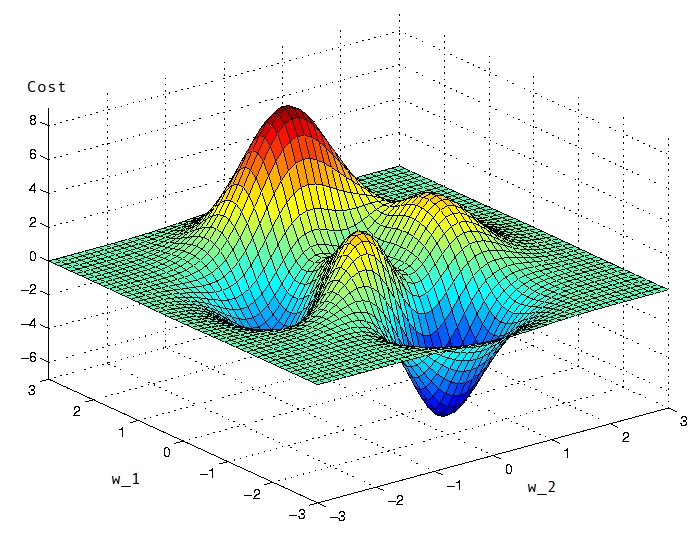
\includegraphics[width=0.9\linewidth]{error_plot}}
\end{figure}

Since the learning rate is such an important parameter, stochastic gradient descent is often enhanced with techniques like momentum, weight decay, and learning rate decay. There are many also variations to stocahstic gradient descent that use adaptive learning rates to decrease training time such as adagrad, lbfgs, adamax, rms-prop, and adam. For examle, lbfgs uses an approximation of the hessian as the learning rate. Interestingly for linear problems, it can be proved that using the hessian as the learning rate finds the optimal weights in one step. While more details on advanced learning methods are not given in this paper, serious deep learning researchers and competitors often use the advanced update algorithms because of the often dramatic increase in performance and decreased training time.

Normally the weights we wish to update from the cost function error are many layers deep. This example follows the model in figure \ref{fig:mlp_ex}, except with a single output instead of two. Therefore, our cost function can be redefined using the previous layer's activations, $\phi_{l}(\mathbf{x}) = \phi_{l}\left(\phi_{l-1}^{T}\mathbf{w}^{l-1}\right) = \phi_{l}\left(a^{l-1}\right)$ and $\phi_{1}(\mathbf{x}) = \mathbf{x}$, and $a^{l-1}$ is considered the activation of layer $l-1$. 

\begin{equation}
    \argmin_{\mathbf{w}} \;\mathrm{RMSE}(\mathbf{x}) = \frac{1}{2}\sum_{N} \left(\mathbf{t} - \phi_{4}\right)^{2}
\end{equation}


\par
To find the weight update for the weights in layer $l$ in a neural network with a total number of layers $L$, we need to take $L - l - 1$ partial derivatives with respect to (w.r.t.) the previous inputs, and one partial derivative w.r.t. to the weights. 
For example, to find the weight updates for the second layer in figure \ref{fig:mlp_ex} we take $4 - 2 - 1 = 1$ derivative w.r.t. to our previous layer's inputs, $\phi_{3}$, and then one derivative w.r.t. to the weights of interest, $\mathbf{w}^{2}$.

\begin{equation}\label{eq:rmse_2}
  \nabla^{2}\mathrm{RMSE}(\mathbf{x}) = \frac{\partial^{2}}{\partial \phi_{3} \partial \mathbf{w}^{2}}\mathrm{RMSE}(\mathbf{x}) = \sum_{N}\left(t - \phi_{4}\right) \times \frac{\partial \phi^{T}_{3}}{\partial \mathbf{w}^{2}}
\end{equation}


\[
  \mathbf{w}_{(t+1)}^{2} = \mathbf{w}_{(t)}^{2} - \eta \times \nabla^{2} RMSE(\mathbf{x})
\]

And like in equation \ref{eq:weight_update}, we have our weight update for $\mathbf{w}^{2}_{(t+1)}$. From equation \ref{eq:rmse_2}, we can see the equation for weight updates is the application of the chain rule. This is significant, because the chain rule will give us insight into computationally effienctly back-propogation.

\newcommand\xbase{-3.95}
\newcommand\ybase{0.7}
\newcommand\hibox{1.2}
\newcommand\wibox{0.88}
\newcommand\tbdis{3.34}
\newcommand\bbdis{3.34}
\newcommand\ybshift{-1.275}
\newcommand\xbshift{-0.45}
\newcommand\xobshift{1.35}
\newcommand\xotshift{1.85}

\begin{equation}\label{eq:chain_rule}
  \begin{tikzpicture}[baseline=(current bounding box.center),thick,scale=0.8, every node/.style={scale=0.8}]
    \node (A) at (0,1.3) {
      \LARGE{$
          \frac{\partial a^{4}}{\partial \mathbf{w}^{1}} =  
          \frac{\partial a^{4}}{\partial a_{2}^{3}}\; \frac{\partial a_{2}^{3}}{\partial a_{3}^{2}}\;\frac{\partial a_{3}^{2}}{\partial \mathbf{w}^{1}} 
          + \frac{\partial a^{4}}{\partial a_{2}^{3}}\; \frac{\partial a_{2}^{3}}{\partial a_{2}^{2}}\;\frac{\partial a_{2}^{2}}{\partial \mathbf{w}^{1}} 
          + \frac{\partial a^{4}}{\partial a_{2}^{3}}\; \frac{\partial a_{2}^{3}}{\partial a_{1}^{2}}\;\frac{\partial a_{1}^{2}}{\partial \mathbf{w}^{1}}
        $}
    };

    \node (B) at (0,0) {
      \LARGE{$
          +\; \frac{\partial a^{4}}{\partial a_{1}^{3}} \;\frac{\partial a_{1}^{3}}{\partial a_{3}^{2}}\;\frac{\partial a_{3}^{2}}{\partial \mathbf{w}^{1}} 
          + \frac{\partial a^{4}}{\partial a_{1}^{3}} \;\frac{\partial a_{1}^{3}}{\partial a_{2}^{2}}\;\frac{\partial a_{2}^{2}}{\partial \mathbf{w}^{1}} 
          + \frac{\partial a^{4}}{\partial a_{1}^{3}} \;\frac{\partial a_{1}^{3}}{\partial a_{1}^{2}}\;\frac{\partial a_{1}^{2}}{\partial \mathbf{w}^{1}}
        $}
    };

    \foreach \Rnumber in {0,...,2} {
      \draw[thick,orange] (\tbdis*\Rnumber + \xbase,\ybase) -- (\tbdis*\Rnumber + \xbase,\ybase + \hibox) -- (\tbdis*\Rnumber + \xbase + \wibox,\ybase + \hibox) -- (\tbdis*\Rnumber + \xbase + \wibox,\ybase) -- (\tbdis*\Rnumber + \xbase,\ybase);
    }

    \foreach \Rnumber in {0,...,2} {
      \draw[thick,green] (\bbdis*\Rnumber + \xbase + \xbshift,\ybase+\ybshift) -- (\bbdis*\Rnumber + \xbase + \xbshift,\ybase+\ybshift + \hibox) -- (\bbdis*\Rnumber + \xbase + \xbshift + \wibox,\ybase+\ybshift + \hibox) -- (\bbdis*\Rnumber + \xbase + \xbshift + \wibox,\ybase+\ybshift) -- (\bbdis*\Rnumber + \xbase + \xbshift,\ybase+\ybshift);
    }

    \foreach \Rnumber/\c in {0/red,1/purple,2/blue} {%
      \draw[thick,\c] (\tbdis*\Rnumber + \xbase + \xotshift,\ybase) -- (\tbdis*\Rnumber + \xbase + \xotshift,\ybase + \hibox) -- (\tbdis*\Rnumber + \xbase + \xotshift + \wibox,\ybase + \hibox) -- (\tbdis*\Rnumber + \xbase + \xotshift + \wibox,\ybase) -- (\tbdis*\Rnumber + \xbase + \xotshift,\ybase);
    }

    \foreach \Rnumber/\c in {0/red,1/purple,2/blue} {%
      \draw[thick,\c] (\bbdis*\Rnumber + \xbase + \xobshift,\ybase+\ybshift) -- (\bbdis*\Rnumber + \xbase + \xobshift,\ybase+\ybshift + \hibox) -- (\bbdis*\Rnumber + \xbase + \xobshift + \wibox,\ybase+\ybshift + \hibox) -- (\bbdis*\Rnumber + \xbase + \xobshift + \wibox,\ybase+\ybshift) -- (\bbdis*\Rnumber + \xbase + \xobshift,\ybase+\ybshift);
    }
  \end{tikzpicture}
\end{equation}

Applying the chain rule to figure \ref{fig:error_plot} yields equation \ref{eq:chain_rule}. Notice how often the chain rule repeats itself. The chain rule computes two partial derivatives three times each, and computes three partial derivatives two times each. Modular back-propogation takes advantage of the redundancy so that each partial derivative needs to only be computed once.

\begin{figure}[H]
  \floatbox[{\capbeside\thisfloatsetup{capbesideposition={right},capbesidewidth=8cm}}]{figure}[\FBwidth]
  {\caption{There are many paths error can travel through the model from the cost function output $a^{4}$. Displayed are the six paths of error required to update a single weight vector between layer $1$ and $2$. Notice that many of the paths go through the same two nodes, three paths for each node in layer $3$. The modular view of back-propogation takes advantage of this repetition.}\label{fig:error_paths}}{\includestandalone[width=0.9\linewidth]{error_paths}}
\end{figure}

\par
To view a neural network from the modular perspective, consider each function as a layer like in figure \ref{fig:single_module} for a single module, and figure \ref{fig:module_nn} for an entire network. We adopt new notation for this discussion as follows. We will use $z_{i}^{l}$ to represent the input of the $i^{th}$ node in the $l^{th}$ layer where there are $L$ total layers, and $z^{l}$ to represent the vectorized input for the entire $l^{th}$ layer. We use $f_{l}(\cdotp)$ to denote an differentiable function that outputs $z^{l+1}$. And we use $C = z^{L}$ for the output of the cost function. A single module needs to be able to perform three computations: 1) a foward pass 2) the partial derivative of previous input w.r.t. current input 3) the partial derivative of the cost w.r.t. previous layer parameters \cite{Freitas}.

\begin{gather}
  1) \; z^{l+1}=f_{l}(z^{l})\label{eq:mod_1} \\
  2) \; \delta_{i}^{l} = \frac{\partial C}{\partial z_{i}^{l}} = \sum_{j} \frac{\partial C}{\partial z_{j}^{l+1}} \frac{\partial z_{j}^{l+1}}{\partial z_{i}^{l}} = \sum_{j}\delta_{j}^{l+1}\frac{\partial z_{j}^{l+1}}{\partial z_{i}^{l}}\label{eq:mod_2}\\
  3) \; \frac{\partial C}{\partial w^{l}} = \sum_{j} \delta_{j}^{l+1}\frac{\partial z_{j}^{l+1}}{\partial w^{l}}\label{eq:mod_3}
\end{gather}

\begin{minipage}{0.37\linewidth}
  \begin{figure}[H]
    \centering
    \includestandalone[width=\linewidth]{module_single}
    \caption{For full functionality of a model a single module of a neural network needs to be able to perform $3$ computations, highlighted in blue.}
    \label{fig:single_module}
  \end{figure}
\end{minipage}\hfill
\begin{minipage}{0.57\linewidth}
  \begin{figure}[H]
    \centering
    \includestandalone[width=0.4\linewidth,angle=270]{module_nn}
    \caption{Pictured is a modular view of a neural network. Notice that only the first layer in this network has weights associated with it. The first layer is the linear layer. The second layer is the ``log-softmax'' layer. The third layer is the ``negative log-likelihood'' function. The second and third layers are fully explained in the logisitc regression section of this paper. If the reader is unfamiliar with their functions, it is advised that they breifly review them.}
    \label{fig:module_nn}
  \end{figure}
\end{minipage}
\vspace{1cm}

Each layer computes their respective $z^{l+1}$ term so that it may pass it to the next layer, and the computation is done in order from input to output. For back-propogation, each layer computes the $\delta^{l}$ term from the output to the input, where $\delta^{L+1}$ is initialized to $1$. Each module can update it's layer's weights (if it has any) whenever the complete set of previous errors, $\delta_{i}^{l+1} \forall i$, is recieved. Relating back to figure \ref{fig:error_paths}, the weight update to $\mathbf{w}^{1}$ can be made once layer $2$ has each of their $\delta_{i}^{2}$. This is how Torch7, a scientific package for machine learning in Lua, computes back-propogation \cite{torch}. For more details on modular back-propogation, see \cite{Freitas}.

Throughout the discussion of the back-propogation, we have been summing from $1$ through $N$ for $N$ training examples. This is computationally inefficient, since the entire training set must pass through the model before any weight updates can be made. This is called the \emph{full-batch} training. In practice, what is done is \emph{mini-batch} training. This is when the $N$ training examples are randomly split into $M$ subsets of $N'$ examples. The error and back-propgation is then computed for a single $M$ subsection of the data, and what is found is that the weight update taken is similar to the update taken when using all $N$ examples. If $N' = 1$ then the learning is called \emph{online-learning}.

\begin{figure}[H]
  \centering
  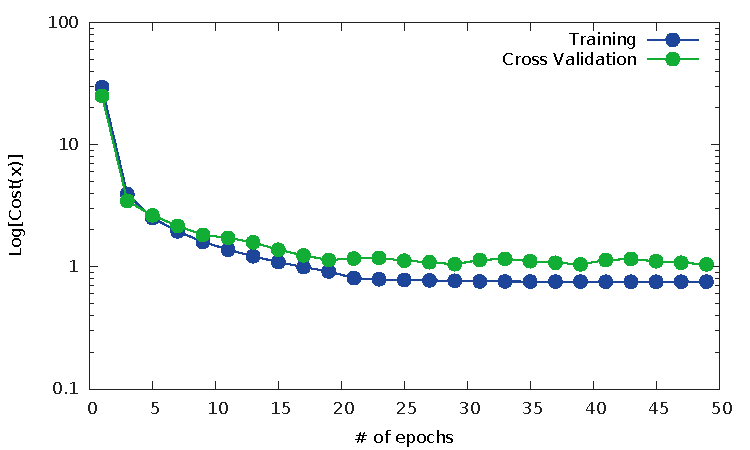
\includegraphics[width=0.5\linewidth]{epoch_mlp}
  \caption{Full-batch versus Mini-batch versus Online learning.}
  \label{fig:learning_size}
\end{figure}


A good practice is also to normalize the data either (a) across each feature, (b) across the entire input vector, or (c) both. For instance, if you want to predict house prices you will likely have features such as number of rooms and number of square feet. We expect the square feet of a house to be much larger numbers (maybe $\approx 1000$) than the number of rooms (maybe $\approx 10$), so it would be wise to normalize the square feet so that the values are not magnitudes different than other features. We can also normalize the entire feature vector. For example, say we have an unrolled image as our input vector where each pixel corrosponds to a feature, and where each pixel can take values from [$1,255$]. It would be smart to normalize the entire feature vector so that each pixel takes value from [$0,1$], so we divide each feature by $255$. The normalization allows us to use more tools. For example if we wanted to train a network to recreate the input, we could now use the Binary Cross Entropy cost function since it's arguments must take values [$0,1$].

\subsection{Logistic \& Multinomial Logistics Regression}

\begin{minipage}{0.52\textwidth}
  \begin{figure}[H]
    \includestandalone[width=\linewidth]{logit}
    \caption{Logistic and multionmial logistic regression is the basic classification for binary and multi-variate classification tasks respectively. Notice how a binary task, yes or no, can be written as both a binary and multi-class problem.}
    \label{fig:logit_nn}
  \end{figure}
\end{minipage}\hfill
\begin{minipage}{0.42\textwidth}
  \begin{figure}[H]
    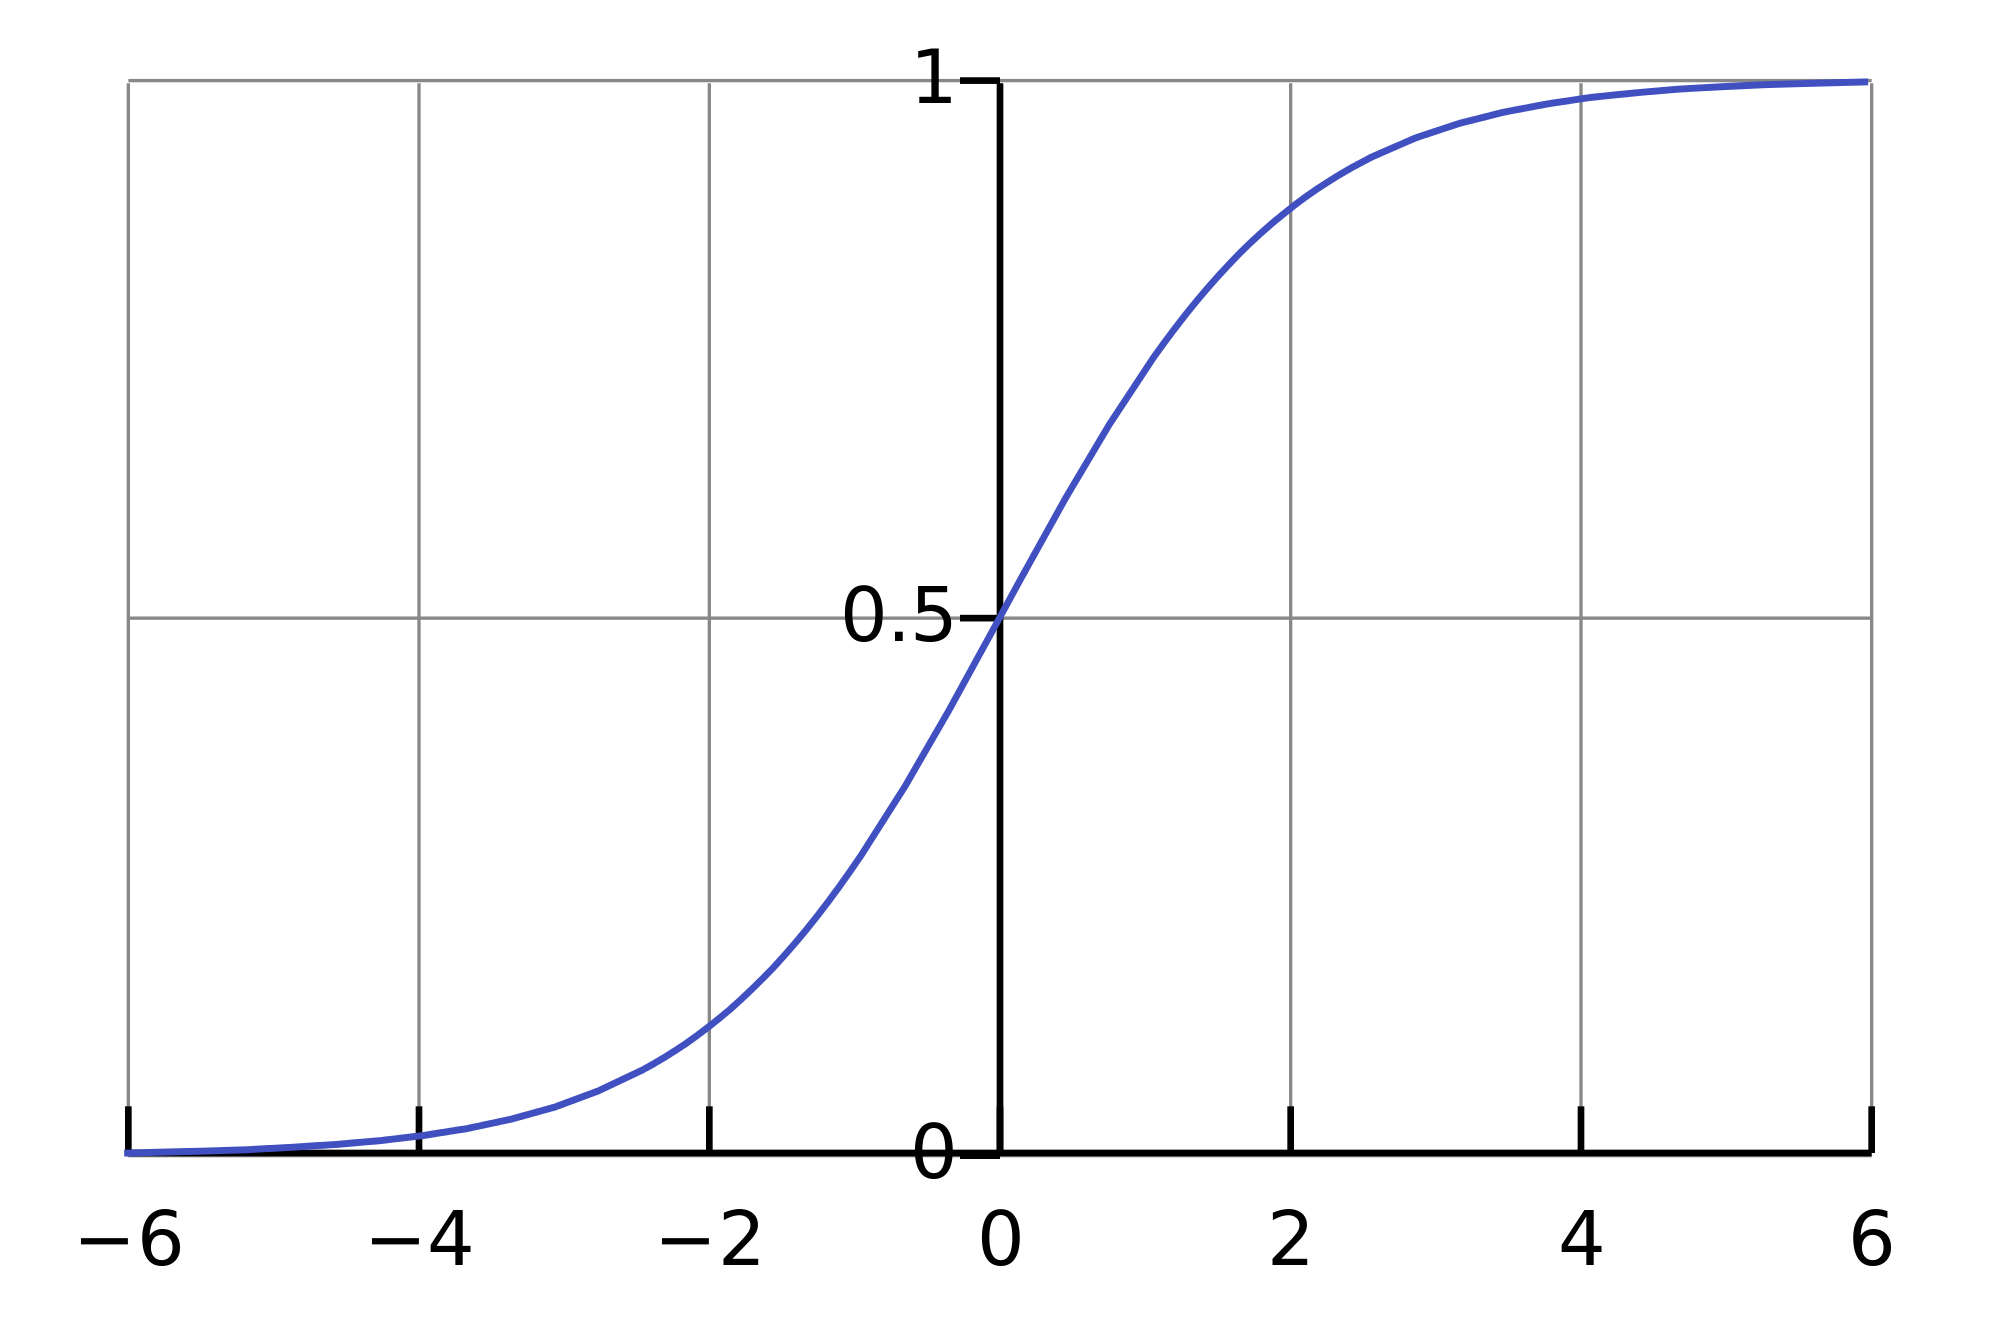
\includegraphics[width=\linewidth]{sigmoid}
    \caption{The sigmoid function ``squashes'' the input argument between $[0,1]$, and is the fundamental building block of classification. This allows us to interpret it's output as probability. Often it is interpreted as the probability of the presence of an arbitrary feature that $\mathbf{w}$ is set to detect.}
    \label{fig:sigmoid}
  \end{figure}
\end{minipage}
\vspace{0.25cm}

Logistic regression can be seen as the left neural network in figure \ref{fig:logit_nn}. The first layer is an input layer consisting of input features. The second layer outputs probability that the input belongs to the class in question. The predictions are the output from the \emph{sigmoid function}, given in equation \ref{eq:sigmoid} and figure \ref{fig:sigmoid}. It squeezes the linear output between $[0,1]$. Note this means our target vector $\mathbf{t}_{i}$ a single scalar value $\in\{0,1\}$. Then it is equivalent to write $\mathbf{t}_{i}$ or $t_{i}$ for the scalar value. This makes probabilist interpretation for binary classification straight-forward. If $\phi(\mathbf{x})$ is some basis function of $\mathbf{x}$, we get: 

\begin{equation}\label{eq:sigmoid}
  \sigma\left(\mathbf{\phi}_{i}^{T}\mathbf{w}\right) = \frac{1}{1+e^{-\mathbf{\phi}_{i}^{T}\mathbf{w}}}
\end{equation}

And formally we can say the output of the sigmoid function is expressed in the following expression.

\begin{equation}
p\left(C_{1}|\mathbf{\phi},\mathbf{w}\right) = \sigma;\; p\left(C_{2}|\mathbf{\phi},\mathbf{w}\right) = 1 - \sigma
\end{equation}

The sigmoid function is interpreted as the posterior probabilty that input $\mathbf{\phi}$ belongs to class $C_{1}$ or $C_{2}$. Using Baye's Rule we get:

\begin{equation}
   \sigma\left(\alpha\right) = P\left(C_{1}|\mathbf{\phi}\right) = \frac{P\left(\mathbf{\phi}|C_{1}\right)P\left(C_{1}\right)}{P\left(\mathbf{\phi}|C_{1}\right)P\left(C_{1}\right) + P\left(\mathbf{\phi}|C_{2}\right)P\left(C_{2}\right)}
\end{equation}

\begin{equation}
  \mathbf{\phi}_{i}^{T}\mathbf{w} = \ln\left(\frac{P\left(\mathbf{\phi}|C_{1}\right)P\left(C_{1}\right)}{P\left(\mathbf{\phi}|C_{2}\right)P\left(C_{2}\right)}\right)
\end{equation}


Note that $\alpha$ depends on a linear combination of the input and parameters from the class-conditional densities. This is why logistic regression is sometimes referred to as a linear classifier despite of it's use of the sigmoid non-linear function. 

Model predicitons are then fed into a cost function to compute the error. The cost function for logistic regression is the \emph{negative-log likelihood} function (N.L.L.). This function relates to the statistical method called \emph{maximum likelihood estimation} (M.L.E.).

Equation \ref{eq:prod_bern} is also known as the likelihood function of $\mathbf{t}$. Our goal is to find the set of weights $\mathbf{w}$ which maximize the likelihood function, as the name ``maximum likelihood'' function implies. Often it more convienent to add rather than multiply, and since the $\log\left(\,\cdotp\right)$ function is $1:1$, it is equivalent to maximize the $\log(\text{eq: }\ref{eq:prod_bern})$.

\begin{equation}\label{eq:prod_bern}
  L\left(\mathbf{t},\phi,\mathbf{w}\right) = p\left(\mathbf{t}|\mathbf{\phi},\mathbf{w}\right) = p\left(t_{1},t_{2},\ldots,t_{N}|\mathbf{\phi},\mathbf{w}\right) = \prod_{i=1}^{N}\sigma^{t_{i}}\left(1-\sigma\right)^{1-t_{i}}
\end{equation}

\begin{equation}
  l\left(\mathbf{t},\phi,\mathbf{w}\right) = \ln\left(p\left(t_{1},t_{2},\ldots,t_{N}|\mathbf{\phi},\mathbf{w}\right)\right) = \sum_{i=1}^{N}t_{i}\ln\left(\sigma\right) - \left(1-t_{i}\right)\ln\left(1-\sigma\right)
\end{equation}

In machine learning our goal is to minimize a cost function. Therefore, to make the interpretation of the function be more closely related to the ``cost'' of our model, we negate the function. Finally, the negative log-liklihood function is given by:

\begin{equation}
  N.L.L.\left(\mathbf{t},\phi,\mathbf{w}\right) = -l\left(\mathbf{t},\phi,\mathbf{w}\right) = -\sum_{i=1}^{m}\ln\left(p\left(t_{i}|\phi,\mathbf{w}\right)\right) = \sum_{i=1}^{N}t_{i}\ln\left(\sigma\right) - \left(1-t_{i}\right)\ln\left(1-\sigma\right)
\end{equation}

The negative log-likelihood criterion is widely popular partially because of it's many interpretations. For a two class case using a single sigmoid unit, like the example above, the negative-log likelihood is also called the \emph{binary cross-entropy} (B.C.E). The negative log-likelihood loss function measures a sudo-distance between the distibutions $Y$ and $\hat{Y}$. More exactly, minimizing the N.L.L. is equivalent to minimizing the Kullback-Leibler Divergence \cite{Freitas}. We say that the N.L.L. function can be thought of as measuring the entropy, or the amount of information our input $\left(\mathbf{x}_{i},\mathbf{t}_{i}\right)$ gives us about our model's accuracy \cite{Freitas}. The more ``information'' we recieve, the more inaccurate our model. More details on the topics of the Kullback-Leibler Divergence and entropy of a random variable are beyond the scope of this paper, however a serious machine learning student should spend time learning about them.


For multiclass cases we use multinomial logistic regression. We change our probability distribution of $\mathbf{t}$ from following a Bernoulli distribution, to following a Multinomial distribution. Therefore, instead of the sigmoid function we use the \emph{soft-max} function. Let $z_{i} = \phi^{T}\mathbf{w}_{i}$, then the multinomial logistic regression neural network seen on the left in figure \ref{fig:logit_nn} can be written as:

\begin{equation}
  \mathbb{I}_{i}\left(\mathbf{q}_{j}\right) =
  \begin{cases}
    1 & \text{if } q_{j,i} = 1\\
    0 & \text{otherwise}
  \end{cases}
\end{equation}

\begin{equation}\label{eq:softmax}
  \text{Soft-Max}\left(\mathbf{t},\phi,\mathbf{w}\right) = 
  \begin{cases}
    \pi_{1} = \frac{e^{z_{1}}}{e^{z_{1}} + e^{z_{2}}} & \mathrm{if\;}\mathbf{t}_{i}\in class\;1\\
    \pi_{2} = \frac{e^{z_{2}}}{e^{z_{1}} + e^{z_{2}}} & \mathrm{if\;}\mathbf{t}_{i}\in class\;2
  \end{cases}
  =
  \pi^{\mathbb{I}_{1}(\mathbf{t}_{i})}_{1} + \pi^{\mathbb{I}_{2}(\mathbf{t}_{i})}_{2}
  = \sum_{j=1}^{j=k}\pi^{\mathbb{I}_{j}(\mathbf{t}_{i})}_{j}
\end{equation}

At the end of the equalities we see the summation form of the soft-max function, which will hold for any number of $k$ classes, where $k = 2$ for the example equation above. The soft-max equation then redefines the multiclass version of equation \ref{eq:prod_bern} as:

\begin{equation}\label{eq:prod_mult}
  L\left(\mathbf{t},\phi,\mathbf{w}\right) = p\left(\mathbf{t} | \phi, \mathbf{w}\right) = \prod_{i=1}^{N} \sum_{j=1}^{K}\pi_{j}^{\mathbb{I}_{j}\left(\mathbf{t}_{i}\right)}
\end{equation}

Again, we wish to take the log of the function so that we sum instead of multiply:

\begin{equation}\label{eq:ln_prod_mult}
  l\left(\mathbf{t}_{i},\phi,\mathbf{w}\right) = \ln\left(p\left(\mathbf{t}|\phi,\mathbf{w}\right)\right) = \sum_{i = 1}^{N}\ln\left(\sum_{j=1}^{K}\pi_{j}^{\mathbb{I}_{j}\left(\mathbf{t}_{i}\right)}\right) = \sum_{i=1}^{N}  \sum_{j=1}^{K} \mathbb{I}_{j}\left(\mathbf{t}_{i}\right) \ln\left(\pi_{j}\right)
\end{equation}

Since we defined $\mathbf{t}_{i}$ to be a member of only one class, the $\ln\left(\text{sum}\right)$ at the end of equation \ref{eq:ln_prod_mult} simplifies to the double sum at the end of the equatlity. And the cost function can be redefined as the \emph{log soft-max} criterion given as:

\begin{equation} \label{eq:cross_entropy}
  \text{Log Soft-max}\left(\mathbf{t}_{i},\phi,\mathbf{w}\right) = - \sum_{i=1}^{N} \mathbb{I}_{1}\left(\mathbf{t}_{i}\right)\ln\left(\pi_{1}\right) + \mathbb{I}_{2}\left(\mathbf{t}_{i}\right)\ln\left(\pi_{2}\right) = - \sum_{i=1}^{N}  \sum_{j=1}^{K} \mathbb{I}_{j}\left(\mathbf{t}_{i}\right) \ln\left(\pi_{j}\right)
\end{equation}

Note that $\pi_{k} \neq 0$ since $e^{z} > 0$. 

This is the complete formulation of logistic regression and multinomial logistic regression in a neural network framework. The weight vectors are found iteratively using back-propogation, just like in a regular neural network.

\subsection{Convolutional Neural Network}

\begin{figure}[H]
  \includestandalone{conv_header}
  \caption{Each color is an instance of a single filter striding across the input image. Each of the filter indicies are multiplied with the corresponding indicies in the image, i.e. the dot product is computed. In this example, the filter has a size of $3\times3$ with a stride of $1$ and the original input image has $1$ row and $1$ column of zero padding. The convolved image is then spatially pooled in $2\times2$ regions to create the final output from our convolution layer.}
  \label{fig:conv_net}
\end{figure}

\par
A convolutional neural network, or ConvNet, is a bona fide method for machine learning tasks including classification and natural language processing \cite{Lecun98}\cite{alexnet}\cite{residual_cnn}\cite{oxford_vgg}\cite{nlp_cnn}. While they were popularized in the $1990$'s \cite{Lecun98}, convolutional nerual networks rose in popularity after Alex Krizhevsky's 2012 Imagenet competiton victory, in which his classification accuracy is $16.4\%$, while the next best accuracy was $26.1\%$ \cite{ILSVRC15}\cite{alexnet}. The standard in today's networks often begin using variations of convolutional layers, so understanding this feature extraction step is an important tool for modern machine learning techniques.

\par
For a discrete signal, which is often the case in machine learning, convoluton between an input signal $x(t)$ and a filter $h(t)$ is given by:

\begin{equation} \label{eq:conv_def}
  x(t) * h(t) = \sum_{\tau=-\infty}^{\infty}h(\tau)x(t-\tau) = \sum_{\tau=-\infty}^{\infty}x(\tau)h(t-\tau)
\end{equation}

This is often thought of as a ``flip-and-shift'' operation. Be careful with the ``flip'' part of the ``flip-and-shift''. Intuitively it might not seem important, but without the ``flip'', convolution become correlation. Indeed many authors use the correlation or convolution, and while they are similar they are not the same thing. From a systems engineering perspective, convolution can be thought of as sending a signal $x(t)$ through a linear time-invariant (or more simply a ``well behaved'') system. Many courses devote ample classtime explaining the topic, and there are many great free online resources to learn more \cite{joyofconv}. However, in this introductory text we will simply take the convolutional layer as feature extraction based on the assumption that nearby pixels are correlated with one another. 

This assumption makes sense for problems like image classification and natural language processing. We can look at the world around us and see that context gives information for inference, and it makes sense to motivate our model structure by giving them context as well. 

\begin{figure}[H]
  \floatbox[{\capbeside\thisfloatsetup{capbesideposition={right,top},capbesidewidth=5cm}}]{figure}[\FBwidth]
  {\caption{Visual representation of a convolutional filter over an input image. The filter is the $3\times3$, stride is set to $1$, and there is one row and column of zero-padding which is highlighted in red. The binary digit $9$ in the first column is convolved with the filter in the second column. The output of the dot product between the pixels and the filter is shown in the far right image.}\label{fig:conv_ex}}{\includestandalone{conv_conv}}
\end{figure}

The computation of a forward pass in a convolutional layer is similar to the definition given in equation \ref{eq:conv_def}. An input image has dimensions W$\times$H$\times$D, where W, H, and D is the width, height, and depth of the image. A \emph{filter}, or kernal, can be of any size, $H_{F} \times W_{F}$, given it is smaller than the input image. The number of filters, $F$, gives the output of a convolutional layer it's depth. A spatial convolution refers to a 2-D filter, and a volumetric convolution refers to a 3-D filter. The filter weights and input image compute the dot product at each position along the way. Generally convolution is done in the following method. The filter starts in the corner of the input image and steps across one dimension. Once it reasches the end of one dimension, the filter increments across an orthogonal direction just once and runs along the original dimension again. This process repeats for the entire length of the orthogonal direction and for all of the orthogonal dimensions to the original dimension. The filter can skip over pixels along the convolution, and the number of pixels skipped per step is called a \emph{stride}, S. If a filter runs along the entire image in all dimensions, the stride is set to $1$. Inceasing the stride decreases the number of positions the filter visits.

After a filter and image has been convolved, the output can be thought of as an image of features. The output is always equal to or less than the size of the original image, but importantly the size of the ouput can be controlled. The output size of the convolution is a function of stride, image size, filter size, and \emph{zero-padding}. Zero-padding, P, is an extra hyperparameter the user picks to adjust the output size of the convolution. Zero-padding adds zeros to the boarder of the input image, and the convolution runs across the new image of the resulting size. More precisely, zero-padding adds a row or column of zeros to the dimension of the image the padding is desired. In figure \ref{fig:conv_ex} we see paddding in $2$ dimensions, $H$ and $W$. We define the output size of a specific dimension, where $I$ is the dimension of interest relating to the input image (i.e. W, H, or D). If the output of a convolution is 3-D, the depth is referred to as \emph{channels}. The channels are the result of using multiple filters, since the filters will stack to create the depth.

\begin{equation}
  \text{Output Dimension Size I} = \frac{(I - F + 2P)}{S} + 1
\end{equation}

After the output of the convolution is calculated, the convolution is generally passed through a non-linear activation function applied elementwise. A common activation function for this is the ReLU activation function in figure \ref{fig:relu}.

\begin{minipage}{0.47\linewidth}
  \centering
  \begin{figure}[H]
    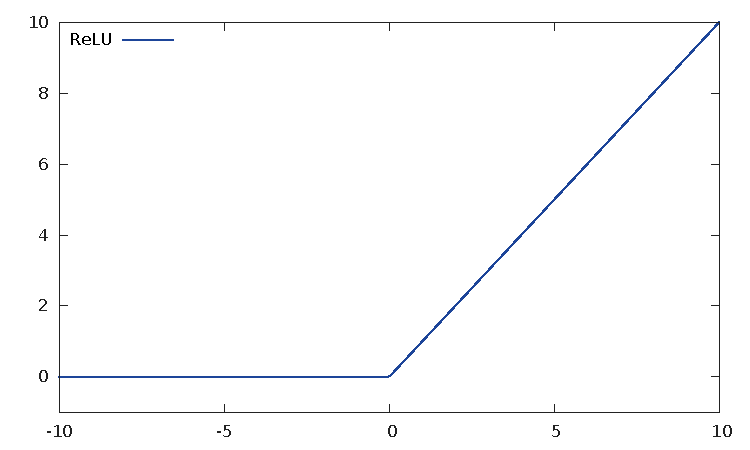
\includegraphics[width=\linewidth]{relu}
    \caption{ReLU activation function given by $\mathrm{ReLU}(x) = \mathrm{max}(0,x)$}
    \label{fig:relu}
  \end{figure}
\end{minipage}\hfill
\begin{minipage}{0.47\linewidth}
  \begin{figure}[H]
    \floatbox[{\thisfloatsetup{capbesideposition={left,top},capbesidewidth=5cm}}]{figure}[\FBwidth]
    {\caption{Max pooling of convolutional output. Each region is annotated}\label{fig:pool_ex}}{
    \includestandalone{conv_pooling}}
  \end{figure}
\end{minipage}\vspace{0.5cm}

The final step of a convolutional layer is \textbf{pooling}. Commonly after a filter is convolved over an image, the output is sent through a non-linearity, and the final step is to ``pool'' the output. This step aims to shrink the resulting image down such that the most important information is retained.

In figure \ref{fig:pool_ex}, current output from the non-linearity (ReLU) is subdivied into smaller regions. The number of regions and their degree of overlap determines the final output size. The major constraint of the regions is that they must be collectively exhaustive, meaning that every element is assigned to at least on region of pooling. Note that there is no significant improvement for overlappign regions \cite{scherer2010evaluation} and is more computationally expensive, so it is often not done in practice.

There are two common types of pooling, \emph{max pooling} and \emph{average pooling}. The max pooling layer simply takes the maximum value from each region. The average pooling layer passes the average value of the region. 

Now that we've computed a complete foward pass of a convolutional layer, we will now dicuss how back-propogation is used in this configuration. The pooling layers are the simplest step. The max pooling layer acts as a gate. The error simply passes through the pooling layer to the non-linearity output, and does not effect the elements that were not chosen during the forward pass. For average pooling, the error is applied by dividing it equally among the number elements in each region. The non-linearity passes error back just like an regular layer, using it's partial derivatives w.r.t. the input to propogate error backward. Given a convolution output with size $H_{F},W_{F},F$, back-propogation is computed by:

\begin{equation}
  \frac{\partial C}{\partial w^{l}_{ijff`}} = \sum_{i`j`f`}\delta^{l+1}_{i`j`f`}\frac{\partial f_{i`j`f`}\left(\mathbf{x}\right)}{\partial w_{ijff`}}
\end{equation}

\subsection{Support Vector Machine}
Fundamentally, classification seperates datasets into different classes depending on the input features. With only $2$ input features, this can be visualized by a linear decision boundarys in figure \ref{fig:svm_bestline}. We can see in the figure that there are many lines that separate the positive and negative class, but which line is the best? Visually it might seem obvious to be the black line, since that is the one that has the most even split between the closest positive and negative data points. In other words, the black line maximizes the margins between both classes.

\begin{figure}[H]
  \centering
  \floatbox[{\capbeside\thisfloatsetup{capbesideposition={right},capbesidewidth=6cm}}]{figure}[\FBwidth]
  {\caption{There are many lines which will classify with $100\%$ accuracy, but some decision boundaries can be considered better than others. The ``$\mcolor{+}$'' corresponds to $\mcolor{+}1$ and the ``$\mcolor[Blue]{-}$'' corresponds to $\mcolor[Blue]{-}1$ on the third dimension not shown. The best line to separate the two classes is the line which cuts exactly between the two classes, leaving the largest margins on either side of the decision boundary (the line).}\label{fig:svm_bestline}}{\includestandalone[width=\linewidth]{svm_bestline}}
\end{figure}

Notice how any of the lines would give us $100\%$ accuracy, and therefore weight updates would stop once any of the lines were reach if we used a negative log-likelihood loss function. A support vector machine is meant to train a model until the ``best'' linear boundary is found. Given that $\mathbf{a} \equiv \left(a_{1},\ldots,a_{N}\right)$ are the Lagrangian constraints for the $N$ training examples of $\mathbf{x}$, the optimal decision boundary is found by using the Lagrangian function below:

\begin{equation}\label{eq:svm_lag}
  L(\mathbf{a}) = \sum_{i=1}^{N}a_{i} - \frac{1}{2}\sum_{i=1}^{N}a_{i}a_{j}\mathbf{t}_{i}\mathbf{t}_{j}k\left(\mathbf{x}_{i},\mathbf{x}_{j}\right)
\end{equation}

For overlapping class distributions, which is frequently the case, equation \ref{eq:svm_lag} is subject to the constraints:

\begin{align}
  0 \leq a_{i} \leq C\label{eq:svm_constraint1}\\
  \sum_{i=1}^{N}a_{i}\mathbf{t}_{i} = 0\label{eq:svm_constraint2}
\end{align}

Solving for the vector $\mathbf{a}$ is a \emph{quadratic programming} problem, and the solution can be found analytically using the SMO algorithm \cite{Platt_smo}. The SMO algorithm is nicely explained in \cite{ng_smo}. Once the Lagrangian constraints are found, the weights $\mathbf{w}$ are calculated using following equation, where $\phi(\cdotp)$ is a basis function:

\begin{equation}\label{eq:svm_weights}
  \mathbf{w} = \sum_{i=1}^{N}a_{i}\mathbf{t}_{i}\phi\left(\mathbf{x}_{i}\right)
\end{equation}
Support vector machines can be seen exactly as a neural network as in figure \ref{fig:svm_nn}, but with a different loss function. We use a \emph{soft-margin classifier} and implement the \emph{hinge-loss function} given by:

\begin{equation}
  \left[\frac{1}{n}\sum^{n}_{i=1}\mathrm{max}\left(0,1 - t_{i}\left(\mathbf{\phi(x_{i})}^{T}\mathbf{w}\right)\right)\right]
  \label{eq:hinge_loss}
\end{equation}

But the above statements work only for linearly seperable datasets. If our data is not linearly separable in the original features space, like the dataset in figure \ref{fig:svm_nonlinear}, we use the method referred to as the \emph{kernal-trick}. The kernal-trick is a specific kind of feature engineering to transform non-linearly separable data into a linearly seperable dataset. The end result of kernals is a new dataset $\mathbf{F} \equiv \left(\mathbf{f}_{1},\ldots,\mathbf{f}_{N}\right)$, where $\mathbf{f}_{i} = \left(f_{1},\ldots,f_{N}\right)$. 

\begin{figure}[H]
  \centering
  \floatbox[{\capbeside\thisfloatsetup{capbesideposition={right},capbesidewidth=7cm}}]{figure}[\FBwidth]
  {\caption{The original data (on the left) can not be classified by a linear decision boundary, so we must use the ``kernal-trick'' to transform the data set into a feature space where the data is linearly seperable (on the right). This image only shows transformation in two of the $7$ dimensions (one for each training example). We used $l_{1}$ and $l_{3}$ as our ``landmarks'', and a guassian kernal with $\sigma^{2} = 1$.}\label{fig:svm_nonlinear}}{\includestandalone[width=\linewidth]{svm_nonlinear}}
\end{figure}

\begin{minipage}{0.47\linewidth}
  \begin{figure}[H]
    \centering
    \includestandalone[width=0.8\linewidth]{svm_nn}
    \caption{The kernalized support vector machine can be seen as the nerual network above, with a special activation function between the first and second layer, which requires no weights. The last layer's output is the ``raw'' output from a linear layer between $\mathbf{f}_{i}$ and $\mathbf{w}$.}
    \label{fig:svm_nn}
  \end{figure}
\end{minipage}\hfill
\begin{minipage}{0.47\linewidth}
  \begin{figure}[H]
    \centering
    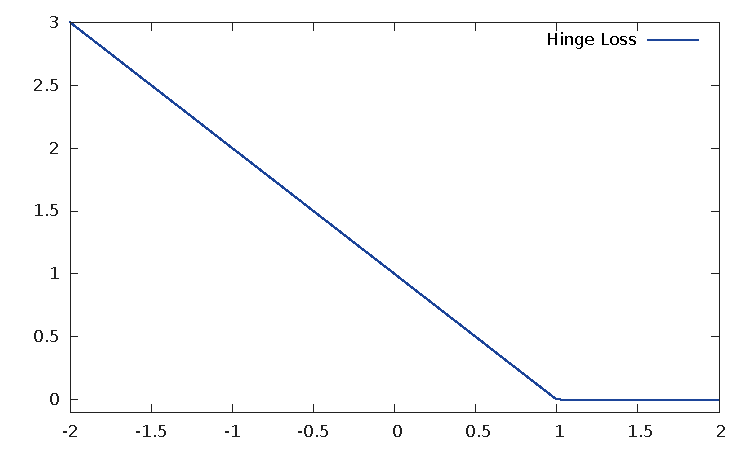
\includegraphics[width=0.8\linewidth]{HingeLoss}
    \caption{The Hinge-Loss function encourages ``+'' examples to be large in magintude and positive, and ``$-$'' examples to be large in magintude and negative.}
    \label{fig:hinge_loss}
  \end{figure}
\end{minipage}\vspace{0.5cm}

In figure \ref{fig:svm_nonlinear}, each example is labeled $\mathbf{x}_{i}$ for the $i^{th}$ training example. The axises are $x_{1}$ and $x_{2}$ for the $1^{st}$ and $2^{nd}$ dimension of each training example $\mathbf{x}_{i}$. Two of the examples, $x_{1}$ and $x_{3}$, have been selected as landmarks $l_{1}$ and $l_{2}$ respectively. 

Note in figure \ref{fig:svm_nonlinear} are we only using $2$ landmarks for educational purposes alone. The proper procedure is to label \textbf{all} of the training examples as landmarks and contiue through the process below. We only graph the result from $2$ landmarks, because we can visualize a $2-D$ plot. A $7-D$ graph is much more challenging to visualize.

For a single landmark  $l_{i}$, our goal is to define a value for a single dimension of each $f_{i}$ vector, $i = 1,\ldots,N$. The indicie of the new vector is arbitrary, but must remain constant for each $\{\mathbf{f}_{i}\}$. Generally, for $N$ training examples there are $N$ dimensions to define for each training example. 

In figure \ref{fig:svm_nonlinear}, the 

engineer new features from our trianing examples $\{\mathbf{x}_{1}\}$ into $f_{1},f_{2},\ldots,f_{m}$ for each $m$ training examples, like in equation \ref{eq:svm_features}. The features are used as coefficients into a linear layer, and are trained on the hinge loss function. We can visualize the kernalized svm as the neural network in figure \ref{fig:svm_nn}.

\begin{gather}
  \text{Start by mapping every } x_{i} \text{ to a landmark } l_{i}\nonumber\\
  \text{For }i \text{ training examples}\nonumber\\
  f_{ik} = \text{similarity}(x_{i},l_{k}) = exp(- \frac{\|l_{i} - x_{k}\|^{2}}{2\sigma ^{2}})\\
  \mathbf{f}_{i} = \left(f_{i1},f_{i2},\ldots,f_{iN}\right), i = 1,\ldots,N\nonumber\\
  \text{Note: } \sigma \text{ is a user defined parameter}\nonumber
  \label{eq:svm_features}
\end{gather}


Supoort vector machines are a powerful tool for analysis. One major benefit of support vector machine's is that their error function is convex, meaning there is a single globally best solution to the function. And even with their shallow depth, they perform well against neural networks, and are still a widely popular algorithm, which achieves test error rate of $0.56\%$ for support vector machines compared with $0.23\%$ for convolutional neural networks\ref{mnist_lecun}.

Despite it's accuracy and popularity, support vector machines have a couple important drawbacks to consider. First is the issue of decision output, and second is the issue of multi-classification. Support vector machines output decisions, not probabilities. The label for a training point $(\mathbf{x},\mathbf{y})$ is $y_{i} = 1$ if $\mathbf{x}$ belongs to the positive class, and $y_{i} = -1$ if $\mathbf{x}$ belongs to the negative class. Therefore, our target $\mathbf{y}$ is no longer a vector, but a single scalar value, whose values are $\{-1,1\}$. The downside to this approach is that we no longer have a probability of our example belonging to the positive or negative class. While we can take the magnitude of the output as the confidence in our label (the furthur from zero, the more confident we are), we still lack the more accurate interpretation from probabilities. And because our output is limited to a scalar value, support vector machines are also constrained to binary classification tasks. We can break up a multi-class classification task into smaller ``one-versus-all'' tasks, where we consider only a single class of being positive and the other classes to be negative. That means for $k$ classes we will have $k$ sets of weights. Input is classified to the classifier with the largest \mcolor{positive} output. These methods can lead to skewed learning, and performance suffers when the number of classes is large. If each example has the same number of $\mathbf{n}$ training examples, then when training each set of weights there are $\mathbf{n}(k - 1)$ negative examples and only $\mathbf{n}$ positive examples.


\subsection{Recurrent Neural Networks}
While recurrent neural networks are a powerful method of supervised learning for sequence prediction, machine translation, and neural turing machines, they do not generally qualify as a classifier. This makes the discussion of recurrent networks challenging in the classificaton setting of the other supervised models. Therefore, we have decided to omit the explaination of recurrent neural networks in the paper.

\section{Unsupervised Learning}

\subsection{K-Means Clustering}
K-means clustering is a common method of unsupervised classification. The motivation is that each sample from a given class will ``live'' inside a similar region in a vector space. Therefore, we can classify our data without ever needing target values. The k-means clustering method is best explained by example. Consider figure \ref{fig:kmeans_data}, where we can clearly see $3$ clusters of data for $3$ different classes. We will use k-means clustering to classify the data.

\begin{minipage}{0.47\linewidth}
  \begin{figure}[H]
    \centering
    \includestandalone[width=0.6\linewidth]{kmeans_data}
    \caption{Pictured is the data for our k-means clustering example. There are $3$ completely separate clusters. While this will give us an easy solution to our clustering problem, frequently in real world datasets class distributions overlap. In these cases, kernal-methods are used (exactly like in support vector machines) to minimize the distribution overlap.}
    \label{fig:kmeans_data}
  \end{figure}
\end{minipage}\hfill
\begin{minipage}{0.47\linewidth}
  \begin{figure}[H]
    \centering
    \includestandalone[width=0.6\linewidth]{kmeans_init}
    \caption{Here we have initialized $k = 3$ clusters. The number of centroids and their initialization is crucial for quality results.}
    \label{fig:kmeans_init}
  \end{figure}
\end{minipage}\vspace{0.5cm}

The first step in k-means is to initialize $k$ clusters, or centroids. In other words, we define $\mathbf{c}_{i}$ for $i = 1,\ldots,k$. In this example, we initialize $3$ clusters as seen in figure \ref{fig:kmeans_init}. However, this is a smart guess we were able to make by simply graphing the data. The data is usually in a higher dimension, such that it is not possible to plot. Clearly, there must be a robust technique to estimate the number of clusters in the dataset. But if the technique fails, it can lead to results that have a different number of centroid than actual clusters in the data. This situation can be seen in figure \ref{fig:kmeans_2or3}.

\underline{TODO:} So how do we find a good number of $k$ centroids?

Ideally data points within a cluster have a small differences, relative to the difference to data points in different clusters. This can be used to check how well our data is clustered. 

\underline{TODO:} How do we initilized k-means?

After the number of centroids is determined and the $k$ clusters have been initalized, we assign every training example to a cluster. This can be seen using colors in figure \ref{fig:kmeans_assignment}. After the assignment, the clusters are moved to the mean location of the assigned data examples. This cycle repeats until convergence.

The cycle is:
\begin{enumerate}
 \item assign training examples
 \item compute and move to the mean location 
\end{enumerate}
When finished, determine if any centroids are assigned to the same cluster.


\begin{minipage}{0.47\linewidth}
  \begin{figure}[H]
    \centering
    \includestandalone[width=0.6\linewidth]{kmeans_assignment}
    \caption{Every training example is assigned to the closest k cluster. The computation for distance can vary, but the Euclidean distance is common.}
    \label{fig:kmeans_assignment}
  \end{figure}
\end{minipage}\hfill
\begin{minipage}{0.47\linewidth}
  \begin{figure}[H]
    \centering
    \includestandalone[width=0.6\linewidth]{kmeans_move}
    \caption{The k clusters move to the mean location of the assigned data-points.}
    \label{fig:kmeans_move}
  \end{figure}
\end{minipage}\vspace{0.5cm}

\begin{minipage}{0.47\linewidth}
  \begin{figure}[H]
    \centering
    \includestandalone[width=0.6\linewidth]{kmeans_2or3}
    \caption{Are there $2$ or $3$ clusters? It is hard for a user to determine without looking at a graph. Computing how well the data is ``clustered'' can be used to determine the initial number of $k$ means. After convergence, corrections can be made to determine if different centroid are assigned to the same cluster.}
    \label{fig:kmeans_2or3}
  \end{figure}
\end{minipage}\hfill
\begin{minipage}{0.47\linewidth}
  \begin{figure}[H]
    \centering
    \includestandalone[width=0.6\linewidth]{kmeans_final}
    \caption{This is the final result of the k-means algorithm. We can clearly see that we have successfully assigned each of the training example to separate classes. Using the dataset, we can now assign the meaning to the clusters.}
    \label{fig:kmeans_final}
  \end{figure}
\end{minipage}\vspace{0.5cm}

But clustering techniques can not solve all problems. The data must be well clustered for k-means classification to work. In fact, we can determine how well data is clustered by using the ``blhasadfasdfa''. For example, we can use the dispersion index of each cluster give in equation \ref{eq:disp_index}, where $\hat{\sigma^{2}}$ is the variance of the data, $\hat{\mu}$ is the mean, and $i = 1,\ldots,N$.

\begin{equation}\label{eq:disp_index}
  \mathrm{D}_{i} = \frac{\hat{\sigma^{2}}}{\hat{\mu}}
\end{equation}

\begin{equation}\label{eq:kmeans_cost}
  J = \sum_{i=1}^{k}\sum_{\mathbf{x} \in \mathbf{c}_{i}}\|\mathbf{x} - \mathbf{c}_{i}\|^{2}
\end{equation}

K-means custering can be seen as minimizing equation \ref{eq:kmeans_cost}. The mathematical forumation of the algorithm can be seen in algorithm \ref{alg:kmeans}.

We can see that clustering provides a good method to classify data without using data targets. It is important to realize that k-means cannot be applied blindly to datasets, and the ``clusteredness'' of the data should be considered. The importance of finding the proper number of clusters $k$ and proper initialization is crucial to having an effective k-means algorithm.

\begin{algorithm}[H]
  \caption{K-Means Clustering
    \label{alg:kmeans}}
  \begin{algorithmic}[1]
    \State Given input that is \textbf{D} dimensional, we begin by initializing $k$ centroids randomly in a \textbf{D} dimensional vector space.
    \State $s_{i},i=1,\ldots,k$ is an empty set to contain the appropriate training examples assigned to the cluster $\mathbf{c}_{i}$.
    \For{\# iterations \emph{or} until convergence}
    \State \underline{Assignment Step:} Each of the data samples $\mathbf{x}_{j}$, $j=1,\ldots,N$ are assigned to the closest cluster $\mathbf{c}_{i}$ determined by a distance metric. In this example, we will use the Eucliean distance.
    
    \begin{equation}
      \mathbf{x}_{j} \in \{s_{i} : \| \mathbf{x}_{j} - \mathbf{c}_{i} \|^{2} \leq \| \mathbf{x}_{j} - \mathbf{c}_{m} \|^{2} \forall m, m \in \{1,\ldots,k\}\}
    \end{equation}

    \State \underline{Update Step:} In this step, the value of each of the data samples within each cluster assignement is averaged. The cluster is then moved to the average of the data samples. Note the $|A|$ notation denotes the cardinality of the set $A$, and returns the number of elements within the set.

    \begin{equation}
      \mathbf{c}^{t+1}_{i} = \frac{1}{|s^{t}_{i}|}\sum_{\mathbf{x} \in s^{t}_{i}} \mathbf{x}_{j}
    \end{equation}


    \EndFor
    \State \textbf{end}
  \end{algorithmic}
\end{algorithm}

\subsection{PCA}
PCA is an algorithm that uses the variance in the dataset to find an optimal linearly compression. Given data in dimension \textbf{D}, PCA maps the data to dimension $\mathbf{\hat{D}}$.
PCA is motivated by the face that information in the data is sometimes redundant, or useless for classification tasks. For example, consider building a classifier between a car, bike, and unicycle. Knowing that a data sample has a seat does not help us predict which class the sample belongs to. What does help is knowing about the attributes which change the most across your dataset. For instance, knowing that the training example has $4$ wheels tells you that your object is a car. Reducing redundant information can greatly reduce computation costs, and more succinctly summarize your data.

\begin{minipage}{0.47\linewidth}
  \begin{figure}[H]
    \centering
    \includestandalone[width=0.6\linewidth]{pca_bad}
    \caption{This is a bad direction to compress the data in, since our variability in the data is low. Notice how the red dots on the baseline are compact. Our reconstruction using the resulting red dots would be poor.}
    \label{fig:pca_bad}
  \end{figure}
\end{minipage}\hfill
\begin{minipage}{0.47\linewidth}
  \begin{figure}[H]
    \centering
    \includestandalone[width=0.6\linewidth]{pca_best}
    \caption{This is the best direction to compress the data. Clearly we have maximized the variability. Note how the line that captures the most variance also satisfies the least-squares solution for this data. Think back to high-school when you talked about the $r^{2}$ term. Linear regression is how much variance is explained by the data, which is captured in the $r^{2}$ term.}
    \label{fig:pca_best}
  \end{figure}
\end{minipage}\vspace{0.5cm}

Since PCA is a set algorithm, we will explaine each step and the intution behind them. First perform mean normalization of the data. This will ``center'' the data around the axis. You can think of this as setting the y-intercept to zero. PCA analysis requires \textbf{two} items: $1$) the direction vectors of maximum variance $\mathbf{U} \equiv \left(\mathbf{u}_{1},\mathbf{u}_{2},\ldots,\mathbf{u}_{\mathbf{\hat{D}}}\right)$, and $2$) the value of the ``red'' dots $\mathbf{s}_{i}$ as seen in figure \ref{fig:pca_best}.

In order to compute $1$ and $2$ for PCA, we must know what eigenvectors and eigenvalues are. Look at equaton \ref{eq:eigen} below. If $\mathrm{A}$ is some $n \times n$ matrix, then $\nu$ is a $n \times 1$ matrix call the \emph{eigenvector} and $\lambda$ is a scalar term called the \emph{eigenvalue}. There are sometimes multiple eigenvectors and eigenvalues for a given matrix $\mathrm{A}$.

\begin{equation}\label{eq:eigen}
  \mathrm{A}\nu = \lambda\nu
\end{equation}

After mean normalizing the data, we must compute the eigenvalues and eigenvectors for the covariance matrix of the data. The covariance matrix is defined in equation \ref{eq:cov_mat}. The direction of greatest variance is the eigenvector with the largest corresponding eigenvalue. Therefore the vectors $u_{i}$ are given by thes eigenvectors $\nu$. This satifies step $1$. To compress the data to dimension $\mathbf{\hat{D}}$, we keep the eigenvectors $\nu_{l}$ correpsonding to the largest eigenvalues, $\lambda_{l}$, for each dimension in $\mathbf{\hat{D}}$. This means we through elimenate the dimensions with low variance, and the vectors $\mathbf{u}_{i} \in \mathbf{U}$ are the eigenvectors pointing in the direction of highest variance.

\begin{equation}\label{eq:cov_mat}
  \Sigma(\mathbf{X}) = \frac{1}{N}\sum_{i=1}^{N}\mathbf{x}_{i}^{T}\mathbf{x}_{i} = 
  \begin{bmatrix}
          \mathrm{var}(x_{1}) & \mathrm{cov}(x_{1},x_{2}) & \ldots & \mathrm{cov}(x_{1},x_{n}) \\
          \mathrm{cov}(x_{2},x_{1}) & \mathrm{var}(x_{2}) & \ldots & \mathrm{cov}(x_{2},x_{n}) \\
          \mathrm{cov}(x_{n},x_{1}) & \mathrm{cov}(x_{n},x_{2}) & \ldots & \mathrm{var}(x_{n},x_{n}) \\
  \end{bmatrix}
\end{equation}

To compute step $2$, calculating the $\mathbf{s}_{i}$, we need to calculate the projection of the original data onto the $u_{i}$ pointing in the direction of maximum variance. The formula is given in equation \ref{eq:pca_nvals}. Remeber that $\mathbf{U}^{T}$ is a $\mathbf{\hat{D}} \times \mathbf{D}$ matrix, and $\mathbf{x}_{i}$ is a $\mathbf{D} \times 1$ vector. Therefore the final output is a $\mathbf{\hat{D}} \times 1$ vector.

\begin{equation}\label{eq:pca_nvals}
  \mathbf{s}_{i} = \mathbf{U}^{T}\mathbf{x}_{i}
\end{equation}

PCA is an excellent linear compression algorithm. However, linear systems are limited in power. In the next section we will look at auto-encoders, which is a non-linear method of data compression.

\subsection{Auto-Encoders}

\begin{minipage}{0.47\linewidth}
  \begin{figure}[H]
    \centering
    \includestandalone[width=0.6\linewidth]{autoenc_nn}
    \caption{This figure represent the architecture of an auto-encoder. Auto-encoders are simply a special case of neural networks. They create low-dimensional, non-linear representations of data.}
    \label{fig:autoenc_nn}
  \end{figure}
\end{minipage}\hfill
\begin{minipage}{0.47\linewidth}
\end{minipage}\vspace{0.5cm}

Auto-encoders provide a non-linear method of data compression.


\section{Hardware and Platform}
\subsection{GPU Performance}
The computationally intensive iterative training of process is a limiting factor in creating completely trained machine learning models. There are two popular solutions to this constraint. One is to use \emph{distributed computing}. The motivation behind distributed computing is to spread the computation among numerous computers, or a computer cluster. This emulates a powerful computer, where no one computer is powerful by themselves. Computer clusters require specialized software, such as Apache Hadoop, to manage distrubtion of data. Running machine learning processes on across a computer cluster requires more software, like the Apache Spark API.

The other method to deal with the computational intensity of training is utilizing a \emph{Graphical Processor Unit} or \emph{GPU}. GPU's are a standard for any serious deep learning research. Alex Krizhevsky's 2012 milestone work on ImageNet utilized the power of parallel GPU's for training \cite{alexnet}. Today NVIDIA creates many popular deep-learning GPU's including the current reigning non-commercial GPU champion, the GeForce GTX GeTitan X pictured in figure \ref{fig:titanx}. For more information on GPU's, visit my collegue's webpage \cite{Karan}.

\begin{figure}[H]
  \floatbox[{\capbeside\thisfloatsetup{capbesideposition={right},capbesidewidth=8cm}}]{figure}[\FBwidth]
  {\caption{The NVIDIA GeForce GTX Titan X is a powerful non-commercial GPU. This GPU boasts $3072$ Cuda cores, $1000$ MHz base clock, $1075$ boost clock, $7$ Gbps memory clock, $12$ GB of GDDR5, and $336.5$ GB/sec memory bandwidth. The retail value of a single Titan X is around $\$1000$, and often deep learning researchers and competitors will purchase a computer with $4$ of them.
    }\label{fig:titanx}}{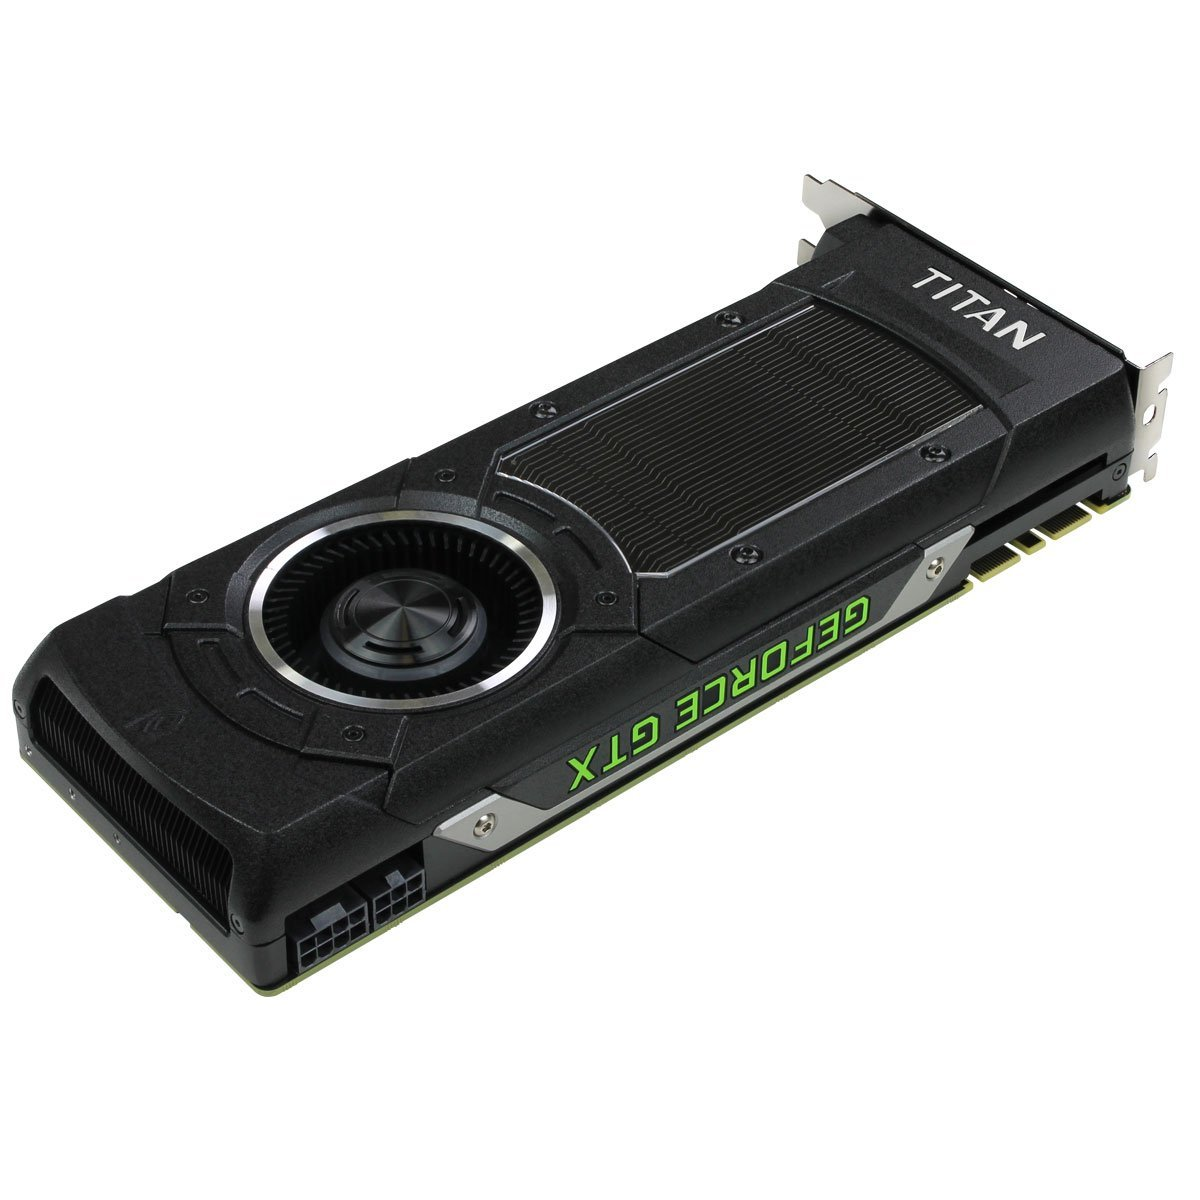
\includegraphics[width=0.65\linewidth]{titanx}}
\end{figure}


\subsection{Coding Platforms}
There are many option when deciding to code for a machine learning platform. Included are Theono, Tensor Flow, Caffee, Torch7, and many more. Nando de Freitas' Oxford University online courses incorperated Torch7, and there were $6$ practicals using the assignment \cite{Freitas}. Therefore, I used Torch7 for each of my models \cite{torch}. My code for the project is available online at \cite{Kent}.

\section{Data Analysis: MNIST}
\subsection{Classification Results}

\begin{center}
  \begin{tabular}{|c|c|c|c|c|}
    \hline
    Model & Training Error & Testing Error & CV Error & \# Misclassified\\
    \hline
    CNN & $99.99\%$ & $98.74\%$ & $98.69\%$ & $307$ \\
    \hline
    MLP & $99.12\%$ & $96.74\%$ & $96.47\%$ & $1119$ \\
    \hline
    SVM & $99.00\%$ & $96.69\%$ & $96.29\%$ & $1202$ \\
    \hline
    Logit & $91.25\%$ & $88.79\%$ & $88.13\%$ & $6683$ \\
    \hline
  \end{tabular}
\end{center}


\begin{minipage}{0.47\linewidth}
  \begin{figure}[H]
    \centering
    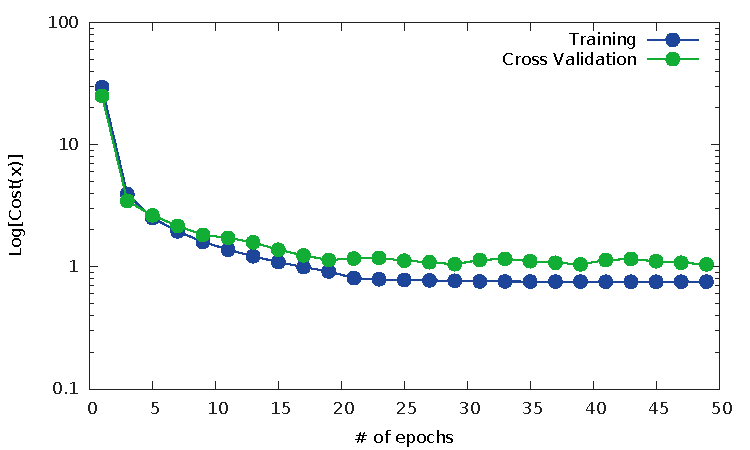
\includegraphics[width=\linewidth]{epoch_mlp}
    \caption{Fitness of Multi-Layer Perceptron.}
    \label{fig:epoch_mlp}
  \end{figure}
\end{minipage}\hfill
\begin{minipage}{0.47\linewidth}
  \begin{figure}[H]
    \centering
    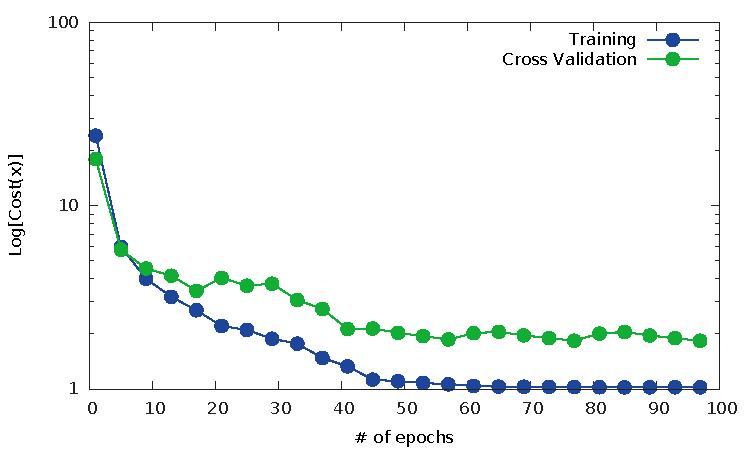
\includegraphics[width=\linewidth]{epoch_logit}
    \caption{Fitness of Logistic Regression}
    \label{fig:epoch_logit}
  \end{figure}
\end{minipage}

\begin{minipage}{0.47\linewidth}
  \begin{figure}[H]
    \centering
    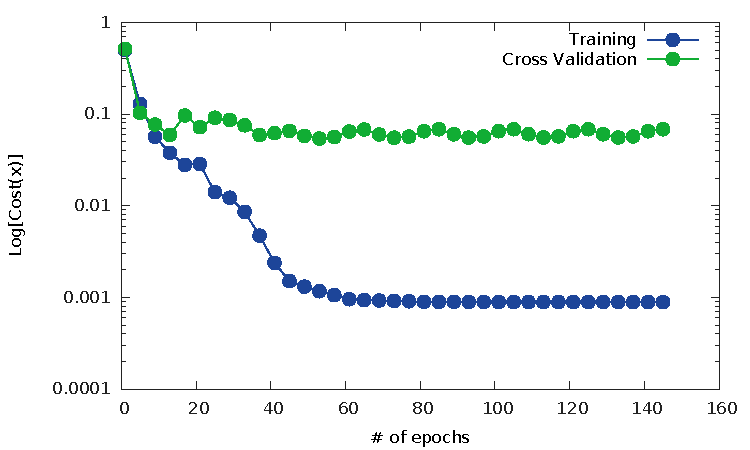
\includegraphics[width=\linewidth]{epoch_cnn}
    \caption{Fitness of Convolutional Neural Network}
    \label{fig:epoch_cnn}
  \end{figure}
\end{minipage}\hfill
\begin{minipage}{0.47\linewidth}
  \begin{figure}[H]
    \centering
    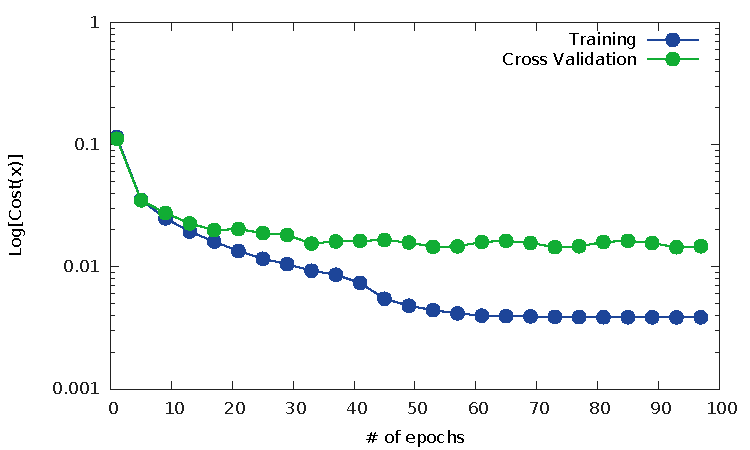
\includegraphics[width=\linewidth]{epoch_svm}
    \caption{Fitness of Support Vector Machine \protect\footnotemark}
    \label{fig:epoch_svm}
  \end{figure}
\end{minipage}

\footnotetext{Loss computed using Hinge-Loss function, instead of NLL like the other $3$ models. Therefore, direction comparision is not appropriate. Instead notice at the convergence, and the differenes between training and cross validation errors.}

\subsection{Features Visualization}

\begin{minipage}{0.47\linewidth}
  \begin{figure}[H]
    \centering
    
\includegraphics[width=0.4\linewidth]{holder}
    \caption{After clustering we can color each cluster to produces an image like this. We can interpret the different colors as the regions that separate the classes.}
    \label{fig:kmeans_image}
  \end{figure}
\end{minipage}\hfill
\begin{minipage}{0.47\linewidth}
  \begin{figure}[H]
    \centering
    
\includegraphics[width=0.4\linewidth]{holder}
    \caption{A compressed representaion of the mnist digits using PCA.  \mcolor{more details on the compression}}
    \label{fig:pca_image}
  \end{figure}
\end{minipage}

\begin{minipage}{0.47\linewidth}
  \begin{figure}[H]
    \centering
    
\includegraphics[width=0.4\linewidth]{holder}
    \caption{A compressed representaion of the mnist digits using auto-encoders. \mcolor{more details on the compression}}
    \label{fig:autoenc_image}
  \end{figure}
\end{minipage}\hfill
\begin{minipage}{0.47\linewidth}
  \begin{figure}[H]
    \centering
    
\includegraphics[width=0.4\linewidth]{holder}
    \caption{The results on the right have the smallest Euclidean distance between the compressed representations of the image on the left and itself. This means that we can interpret the compressed representation as having some correlation to the content of the image.}
    \label{fig:autoenc_fetch}
  \end{figure}
\end{minipage}



\section{Conclusion}



\printbibliography

\end{document}
